%%%%%%%%%%%%%%%%%%% Pruebas
\begin{frame}{Introducción}{Historia...}
	\justifying
        Los \underline{relojes vectoriales} son un tipo de
        reloj lógico propuesto de manera independiente por
        \textit{Colin J. Fidge} y \textit{Friedemann Mattern}
        en 1988.
        
        \begin{center}
          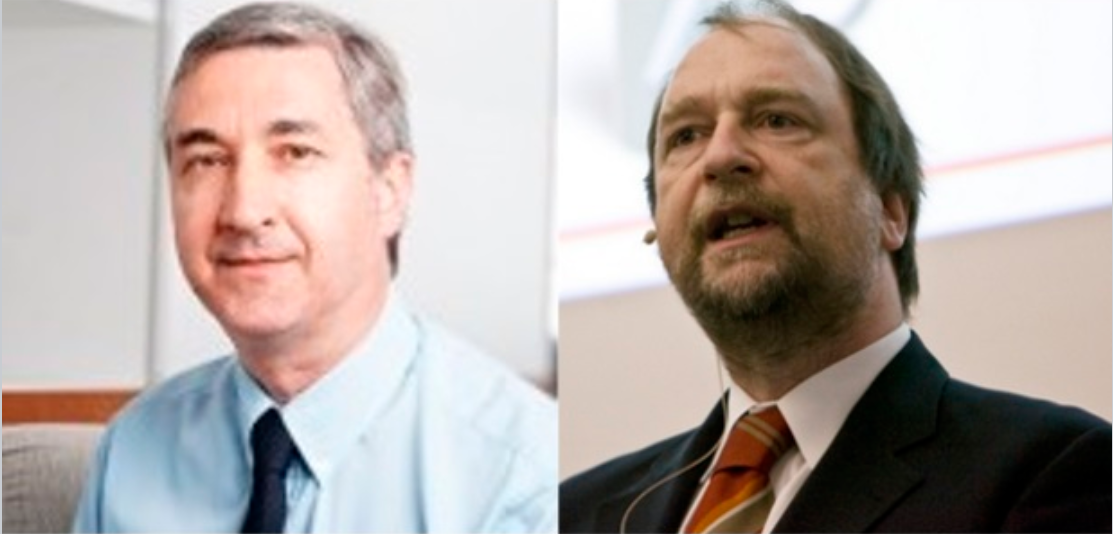
\includegraphics[height = 2cm]{./Imagenes/FidgeAndMattern.png}
        \end{center}
        
        Esta técnica consiste en un mapeo entre eventos en una
        historia distribuida y vectores enteros.
\end{frame}
